\section{OpenFOAM setup and the automated pipeline}
\label{sec:method}

\textbf{Purpose.} Every number in this report depends on a solver recipe, a trim convention and a
convergence gate, and every case reached its number down one automated route. This section fixes
each of them once, so that no result section has to restate them and no two results can rest on
different ones.
\subsection{Solver, boundary conditions and mesh}
\label{sec:setup}
\label{sec:setup:solver}

\textbf{Recipe.} Every value here was read from the recipe folder each case was built from, and
the recipes were confirmed against the built cases \texttt{SWB\_a1p60} and \texttt{CMPB\_a0p87}.
Per-geometry surface and cell counts are in Table~\ref{tab:geom:mesh}.
\textbf{Method.} Both conditions run \texttt{foamRun} under OpenFOAM-org~12~\cite{openfoam},
steady state, SIMPLEC. Condition~CR uses the \texttt{incompressibleFluid} module at
$\nu = \num{1.46e-5}$~m$^2$/s. Cruise uses the \texttt{fluid} module in transonic mode with a
perfect gas. Table~\ref{tab:setup:numerics} gives both setups.

\textbf{Two models, by design.} Condition~CR runs kOmegaSST wall resolved and cruise runs
Spalart-Allmaras wall modelled. The criterion is the drag split: skin friction cancels between
the members of a morph pair, and Spalart-Allmaras is the stronger model on the drag-rise
derivative that does not. \texttt{nutLowReWallFunction} sets $\nu_t = 0$ at the wall and is the
resolved-sublayer condition. Within a condition the model and the wall treatment are uniform.

\textbf{Numerics.} The cruise schemes and solution control are byte-copied from the project's
Onera~M6 case. That case reproduces AGARD AR-138 run 308~\cite{agard138}. Condition~CR runs
limited gradients, a limited surface-normal gradient and one non-orthogonal corrector.

\textbf{Residuals.} Residual targets sit below anything these solves reach. Each run therefore
ends at \texttt{endTime}, and the force gate of Section~\ref{sec:setup:gate} decides. Achieved
residuals are flat rather than falling. Condition~CR reaches $U_x \sim 10^{-9}$ and cruise
$U_x \sim \num{1.8e-7}$.

\begin{table}[htbp]
  \centering
  \scriptsize
  \caption{Discretisation and solution control, read from the two recipe folders and confirmed
  against the built cases. Residual targets are set below anything the solve reaches, so the run
  ends at \texttt{endTime} and the gate of Table~\ref{tab:setup:gate} decides; the achieved
  plateau levels are given alongside. The cruise column serves both $M = 0.78$ states, which
  differ only in freestream state and layer stack.}
  \label{tab:setup:numerics}
  \begin{tabular}{lll}
    \toprule
     & Condition CR & Cruise (early and late) \\
    \midrule
    Module, fluid        & \texttt{incompressibleFluid}, $\nu$ $\num{1.46e-5}$
                         & \texttt{fluid} transonic, $Cp$ $1005$, $Pr$ $0.71$ \\
    Turbulence model     & kOmegaSST & Spalart-Allmaras \\
    $\nu_t$ wall condition & \texttt{nutLowReWallFunction} & \texttt{nutUSpaldingWallFunction} \\
    Gradient             & \multicolumn{2}{l}{Gauss linear, cell limited on $U$ and turbulence} \\
    Convection, $U$      & bounded linearUpwind & linearUpwind \\
    Convection, turbulence & bounded limitedLinear 1 & linearUpwind \\
    Convection, energy   & n/a & \texttt{filteredLinear2 0.2 0} \\
    Laplacian, snGrad    & limited corrected $0.33$ & corrected \\
    $p$ solver           & GAMG $10^{-8}$, relTol $0.01$ & GAMG $10^{-8}$, relTol $0.1$ \\
    $U$, turbulence solver & smoothSolver $10^{-9}$ & GAMG $10^{-8}$, relTol $0.1$ \\
    Non-orth. correctors & 1 & 0 \\
    Relaxation           & $U$ $0.5$, all $0.5$ & $p$ $1$, $U$ $0.9$, $e$ $0.8$ \\
    Residual targets     & $p$ $10^{-9}$, $U$ $10^{-10}$
                         & $p$ $10^{-9}$, $U$ $10^{-10}$, $e$ $10^{-9}$ \\
    Residuals achieved   & $U_x$ $\sim10^{-9}$, $p$ $\sim10^{-8}$
                         & $U_x$ $\sim\num{1.8e-7}$, $p$ $\sim\num{2e-8}$ \\
    \bottomrule
  \end{tabular}
\end{table}

\textbf{Domain.} The domain is free air. One background block spans $60\times30\times60$~m,
which puts the far field $16.4$ semispans out. The root plane is a symmetry plane and the wing
is \texttt{noSlip}. Table~\ref{tab:setup:bc} gives the patch conditions per field.
\textbf{Incidence.} Incidence enters through the freestream vector and the force axes.
Condition~CR runs $U_\infty = (33.991249,\,0,\,0.771369)$~m/s. Early cruise runs
$(233.907340,\,0,\,3.533537)$~m/s. Each case's $\alpha$ is read back from the \texttt{dragDir}
header the solver wrote, never from the case name.

\textbf{Turbulence inflow.} Every case is fully turbulent from the leading edge. Condition~CR
carries $k = \num{1.734e-3}$~m$^2$/s$^2$ and $\omega = 14.25$~s$^{-1}$. That is a turbulence
intensity of $0.10$~per~cent and $\nu_t/\nu = 8.3$. Cruise carries
$\tilde{\nu} = \num{1.3056e-5}$~m$^2$/s, and zero at the wall.

\begin{table}[htbp]
  \centering
  \scriptsize
  \caption{Boundary conditions as built, per patch and field. Condition~CR fixes pressure at the
  outlet and leaves the other far-field patches \texttt{zeroGradient}; the compressible cases use
  the \texttt{freestream} pair on all four far-field patches. Forces are integrated over the
  \texttt{wing} patch alone.}
  \label{tab:setup:bc}
  \begin{tabular}{lll}
    \toprule
    Patch & Condition CR & Cruise (early and late) \\
    \midrule
    \texttt{wing}   & $U$ \texttt{noSlip}, $p$ \texttt{zeroGradient}
                    & $U$ \texttt{noSlip}, $p$ \texttt{zeroGradient} \\
                    & $k$ \texttt{kLowReWallFunction}
                    & $T$ \texttt{zeroGradient}, $\tilde{\nu}$ fixed $0$ \\
                    & $\omega$ \texttt{omegaWallFunction}
                    & $\nu_t$ \texttt{nutUSpaldingWallFunction} \\
                    & $\nu_t$ \texttt{nutLowReWallFunction}
                    & $\alpha_t$ \texttt{alphatWallFunction} \\
    \midrule
    \texttt{symmetry} & \texttt{symmetry} & \texttt{symmetryPlane} \\
    \midrule
    \texttt{inlet}, \texttt{topBottom}, & $U$, $k$, $\omega$ \texttt{inletOutlet}
                    & $U$ \texttt{freestreamVelocity}, $p$ \texttt{freestreamPressure} \\
    \texttt{outboard} & $p$ \texttt{zeroGradient}, $\nu_t$ \texttt{calculated}
                    & $T$, $\tilde{\nu}$ \texttt{inletOutlet}, $\nu_t$ \texttt{calculated} \\
    \midrule
    \texttt{outlet} & $p$ \texttt{fixedValue} $0$, $U$ \texttt{inletOutlet}
                    & as the other far-field patches \\
    \bottomrule
  \end{tabular}
\end{table}

\label{sec:setup:mesh}
\textbf{Mesh.} One mesh recipe serves both conditions, and only the prism stack differs. The
surface cell is set by the $1.03$~mm blunt trailing edge, not by wall treatment or Reynolds
number. Refinement level 11 gives a $\num{0.488}$~mm surface cell and $2.11$ cells across the
trailing-edge base. The two recipes agree on wall-face count to three faces in
$5.28\times10^{6}$, which is the measured form of the claim that one recipe serves both
conditions. Table~\ref{tab:setup:mesh} gives the recipe and what was built from it.
\textbf{Layers.} Condition~CR asks 11 layers at a $4.5$~$\mu$m first cell and builds $9.79$ of
them. Early cruise asks 5 at $43.7$~$\mu$m and builds $4.96$ on every cruise mesh; late cruise
asks 5 at $56.1$~$\mu$m and builds $4.97$. Achieved stack heights are $95.2$, $99.5$ and
$99.6$~per~cent of the request, read from each mesh's own log; an achieved stack can only fall
below the request, and every one does. Extrusion covers $97.1$~per~cent of wall faces at
Condition~CR and $99.91$ to $99.93$~per~cent at cruise.

\textbf{Wake boxes and cell cap.} Both conditions carry two Trefftz wake boxes over the aft
wing and near wake, at levels 7 and 6, under a $130$~million cell cap. Every one of the twelve fails three to five \texttt{checkMesh} checks,
drawn from skewness, face tetrahedra, small determinant and concavity, plus a
small-interpolation-weight flag on C's early-cruise mesh alone; maximum non-orthogonality is $72.4^{\circ}$ to
$74.9^{\circ}$.

\textbf{Achieved $y^+$ is the design value.} The stack is sized to put the first-cell top at the
nominal target. OpenFOAM evaluates $y^+$ at the cell centre, so a correct stack reads half the
nominal figure. Condition~CR is designed at $0.541$ and $0.270$, cruise at $80.3$ and $40.1$.
Measured band medians are $0.279$ to $0.302$ and $37.5$ to $41.9$. Both conditions sit on their
design value, and the cruise wall condition is blended across the buffer layer.

\begin{table}[htbp]
  \centering
  \scriptsize
  \caption{Mesh recipe and as-built statistics. Only the layer stack differs between the two
  conditions. Surface cell size is $1.0/2^{11} = \num{0.488}$~mm. Design $y^+$ is quoted at the
  first-cell top and at the cell centre, the centre being where OpenFOAM's \texttt{yPlus} object
  evaluates. Measured $y^+$ is the band median over the five sampled semispan stations of each
  solved trim case, six at Condition~CR and six at early cruise, from the section cuts. The cruise
  column is the early-cruise mesh; late cruise differs only in its first layer.
  Per-geometry cell counts are in Table~\ref{tab:geom:mesh}.}
  \label{tab:setup:mesh}
  \begin{tabular}{lll}
    \toprule
     & Condition CR (wall resolved) & Cruise (wall modelled) \\
    \midrule
    Background        & \multicolumn{2}{l}{$60\times30\times60$~m at $60\times30\times60$ cells, base $1.0$~m} \\
    Surface level     & \multicolumn{2}{l}{11, giving $\num{0.488}$~mm; feature and TE levels also 11} \\
    Distance shells   & \multicolumn{2}{l}{level 8 / 7 / 6 / 5 at $0.030$ / $0.100$ / $0.350$ / $1.200$~m} \\
    Wake, cone, morph & \multicolumn{2}{l}{level 7} \\
    Quality limits    & \multicolumn{2}{l}{non-orthogonality 65 (relaxed 75), skewness 4} \\
    Decomposition     & \multicolumn{2}{l}{192 subdomains, hierarchical} \\
    \midrule
    Layers asked      & 11, first $4.5$~$\mu$m, $r$ $1.450$ & 5, first $43.7$~$\mu$m, $r$ $1.300$ \\
    Stack asked       & $0.586$~mm & $0.395$~mm \\
    Layers achieved   & $9.79$ of 11, $95.2$\,\% of stack & $4.96$ of 5, $99.5$\,\% of stack \\
    Extrusion         & $97.1$\,\% of wall faces & $99.91$\,\% of wall faces \\
    Wall faces        & $\num{5276772}$ & $\num{5276562}$ to $\num{5277084}$ \\
    Max non-orthogonality & $70.19$ to $70.98$ & $74.10$ to $74.86$ \\
    \midrule
    Design $y^+$, top / centre  & $0.541$ / $0.270$ & $80.3$ / $40.1$ \\
    Measured $y^+$, band median & $0.279$ to $0.302$ & $37.5$ to $41.9$ \\
    \bottomrule
  \end{tabular}
\end{table}

\subsection{The automated pipeline}
\label{sec:setup:pipeline}

\textbf{Pipeline.} Figure~\ref{fig:pipeline} is the route from a delivered geometry to a quotable
number, and every case in this report went down it without manual dictionary editing. The shaded
boxes are gates: a surface that is not closed, a mesh outside the quality limits, or a force
history that has not settled stops the case there. Nothing is asserted by the step that was
supposed to cause it. The run card is written from the case, the harvest is written from the run
cards, and every table and figure in this report is regenerated from the harvest by script, with
the checks of Section~\ref{sec:cond:coverage} run before any number is quoted.

\begin{figure}[htbp]
  \centering
  \resizebox{\linewidth}{!}{% The automated pipeline, one case from geometry to a quotable number. \input inside a figure.
% Gates are the shaded boxes: a case that fails one stops there. Boxes carry at most eight words.
\begin{tikzpicture}[
  font=\footnotesize,
  node distance=4mm and 5mm,
  box/.style={draw, rounded corners=1.5pt, align=center, minimum height=8.5mm,
               text width=26mm, inner sep=2pt, line width=0.5pt},
  gate/.style={box, fill=black!10, line width=0.7pt},
  rec/.style={box, fill=blue!7},
  arr/.style={-{Latex[length=2mm]}, line width=0.5pt},
  lab/.style={font=\scriptsize\itshape, text=black!60}
]
% row 1: geometry and mesh
\node[box] (geo)  {OpenVSP geometry\\ \texttt{.vsp3}, STL export};
\node[box, right=of geo] (place) {Scale feet to metres\\ strip non-wing solids, place};
\node[gate, right=of place] (sc) {\texttt{surfaceCheck}\\ closed, one zone, oriented};
\node[box, right=of sc] (mesh) {\texttt{blockMesh} + \texttt{snappyHexMesh}\\ level 11 surface, prism stack};
\node[gate, right=of mesh] (cm) {\texttt{checkMesh}\\ non-orthogonality, skewness};
\node[box, right=of cm] (dec) {\texttt{decomposePar}\\ 192 subdomains};
% row 2: solve and trim
\node[box, below=9mm of dec] (br) {Bracket: three angles\\ \texttt{foamRun} to \texttt{endTime}};
\node[gate, left=of br] (g1) {Convergence gate\\ 200-sample drift and span};
\node[box, left=of g1] (fit) {Lift-slope fit\\ target $C_L$ inside the bracket};
\node[box, left=of fit] (trim) {Trim case\\ solved at the fitted angle};
\node[gate, left=of trim] (g2) {Convergence gate\\ and $|C_L-\mathrm{target}| < 10^{-4}$};
\node[rec, left=of g2] (card) {Run card, JSON\\ checksum, mesh, $y^+$, forces};
% row 3: record
\node[rec, below=9mm of card] (harv) {Harvest\\ \texttt{rans\_forces.json}};
\node[rec, right=of harv] (tab) {Tables and figures\\ regenerated by script};
\node[rec, right=of tab] (gate3) {Report gates\\ tables against data, no narration};
% arrows
\foreach \a/\b in {geo/place, place/sc, sc/mesh, mesh/cm, cm/dec, br/g1, g1/fit, fit/trim, trim/g2, g2/card, harv/tab, tab/gate3}
  \draw[arr] (\a) -- (\b);
\draw[arr] (dec.south) -- (br.north);
\draw[arr] (card.south) -- (harv.north);
% side labels
\node[lab, left=1mm of geo.west, anchor=east] {geometry};
\node[lab, right=1mm of br.east, anchor=west] {solve};
\node[lab, left=1mm of harv.west, anchor=east] {record};
\node[lab, above=0.5mm of sc.north] {gate};
\node[lab, above=0.5mm of cm.north] {gate};
\node[lab, below=0.5mm of g1.south] {gate};
\node[lab, below=0.5mm of g2.south] {gate};
\end{tikzpicture}
}
  \caption{The automated pipeline, one case from geometry to record. Shaded boxes are gates, and
  a case that fails one stops there.}
  \label{fig:pipeline}
\end{figure}
\subsection{Trim convention: every comparison is at matched lift}
\label{sec:cond:trim}
\textbf{Purpose.} Drag is compared at the same lift, not at the same angle of attack. A morphed
wing carries the target lift at a different incidence from the baseline. Comparing the two at one
fixed angle would read a lift difference as a drag difference. This is the single convention the
whole report rests on.

\textbf{Method at Condition~CR.} Three angles bracketing the expected trim are solved to convergence. Three
geometries trim below their first bracket and carry a fourth bracket angle, lower than the other
three. $C_L$ and $C_D$ window means are fitted by least squares through all bracket angles, and
the fit residuals are printed. The trim angle follows from that fit, and a separate trim case is
solved at it: the fourth case run for most geometries, and the fifth for the three that needed an
extra bracket. That solved case is the quotable point, not an interpolation. The target must lie inside the bracket, and an extrapolated
angle is refused.

\textbf{Two details that keep the convention honest.} Incidence is read from each case's own
freestream vector, not from its directory name; \texttt{CMPC\_a0p87} actually runs
$0.8655$~deg. All three bracket cases are asserted to share one operating point, derived from each
case's own density and agreed to $10^{-12}$, before any fit is formed.

\textbf{Method at cruise.} The cruise trims were reached by continuation rather than by
bracketing. Each case converged a first leg at an initial incidence, was nudged in $\alpha$ on its
own lift slope (a prior slope for the first nudge, the secant through its own legs after that),
and continued until $|\Delta C_L| < 10^{-4}$. Each nudge rotates the freestream and the
force-coefficient axes together, and the solved axes are asserted to agree with the trimmed
incidence to $10^{-6}$~deg. Nine of the twelve needed one nudge and three needed two;
Table~\ref{tab:trim:legs} lists every leg. The off-trim legs converged on the same gate as the
trims and are the only points the cruise drag-due-to-lift slopes use.

\begin{table}[htbp]
\centering
\footnotesize
\caption{Every cruise trim leg. $\Delta\alpha$ is the nudge applied after the leg. LCF's third
leg stopped after one iteration and was continued as its fourth, so its legs read 1, 2, 4. Source:
\texttt{data/rans\_forces.json}, \texttt{trim\_history} of each case.}
\label{tab:trim:legs}
\begin{tabular}{lrrrrrrl}
\toprule
Geom. & Leg & Iter. & $\alpha$ (deg) & $C_L$ & $C_L-$tgt (ct) & $C_D$ (ct) & $\Delta\alpha$ (deg) \\
\midrule
\inputrows{sections/gen/tab_trim_legs.tex}
\bottomrule
\end{tabular}
\end{table}

\textbf{Result.} The trim outcome for every geometry and condition is in the performance tables,
Tables~\ref{tab:perf:cr}, \ref{tab:perf:ec} and~\ref{tab:perf:lc}, which carry each trim's
incidence and its lift residual against that condition's own target;
Figure~\ref{fig:cond:clalpha} is the picture of the Condition~CR procedure. The project tolerance
is $|\Delta C_L| < 1\times10^{-4}$, one count of lift, and all eighteen trims are inside it: the
widest is \texttt{LCW\_trim} at $0.895$ counts. Each family's own drag-due-to-lift slope converts
a lift residual into drag, and the largest such bias at any condition is $0.036$ counts, on
\texttt{LCW\_trim}. At cruise six of the twelve slopes rest on a nudge too small to resolve the
slope, under $0.002$ in $C_L$; they are flagged in the data file as fit to the trim residual only,
and they bound it well below $0.1$ counts either way. The same conversion over the six
Condition~CR trims gives at most $0.003$ counts.

\begin{figure}[htbp]
  \centering
  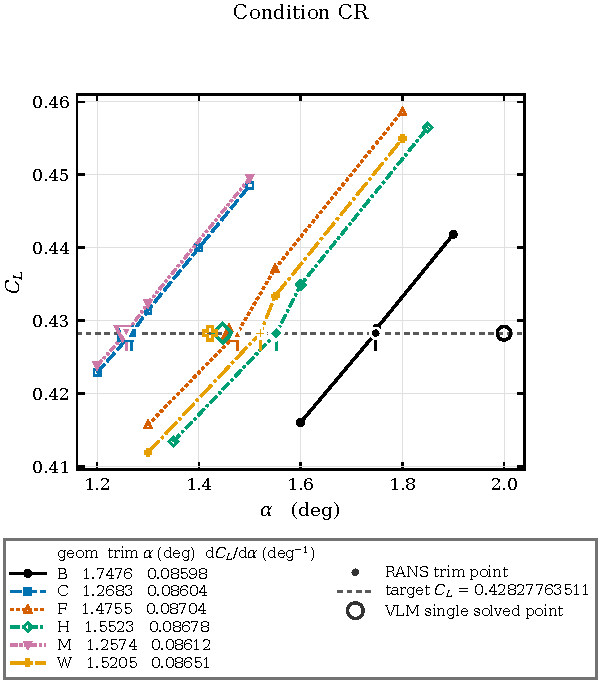
\includegraphics[width=0.40\textwidth]{fig/cl_alpha_condition_CR.pdf}
  \caption{The trim procedure made visible at Condition~CR; the cruise trims were reached by
  continuation and are tabulated in Table~\ref{tab:trim:legs}.
  $C_L$ against $\alpha$ over each family's solved angles, with the target drawn as a dashed
  line and each solved trim case filled. Rings are single-point VSPAERO trims,
  drawn to show agreement on incidence and carrying no lift slope of their own.
  DSO basis, half model, $A_\mathrm{ref} = \num{0.620462}$~m$^2$.}
  \label{fig:cond:clalpha}
\end{figure}

\textbf{Decision.} Every drag count in this report is a difference taken at matched lift, inside
one condition, on one reference frame. The residuals above are worth hundredths of a count of
drag at most, against candidate differences of tenths of a count at Condition~CR and up to fifteen
counts at cruise. The comparison is therefore read as a drag
comparison at fixed lift, with no lift correction applied to any number.

\subsection{Convergence gate}
\label{sec:setup:gate}
\textbf{Method.} A steady SIMPLE solve on this wing limit-cycles about a stationary mean. The
gate is therefore written on the drift of the mean and on the span across the window. It is
evaluated once at the end of each leg, over the last 200 force samples. All three terms must
pass, and the verdict is re-derived from the forces by a second script.
Table~\ref{tab:setup:gate} gives the thresholds and what the 55 cases converged at the
15~September regeneration achieved. \textbf{That set is not the 90 converged cases counted in
Table~\ref{tab:project-scope}}; the rest landed after it. The gate itself is unchanged and every
later case passed it on its own force history. Over the 27 cruise trims and legs that carry every
cruise result in this report, the
achieved values are $C_d$ drift $0.0001$ to $0.0240$~ct (median $0.0022$), $C_l$ drift $0.0037$ to
$0.4007$~ct (median $0.0559$) and $C_l$ span $0.0013$ to $0.8637$~ct (median $0.1223$), all 27
CONVERGED over 200 samples; the widest are first legs, before the nudge, and every trim sits well
inside. What is not claimed is that the tabulated statistics were recomputed over all ninety.

\textbf{Sampling.} 200 samples is a different number of iterations per condition. Condition~CR
writes forces every fifth time step and cruise every step. On a leg ending at \texttt{endTime}
$4000$, which is 46 of those 55, the windows therefore span $t = 3005$ to $4000$
and $t = 3801$ to $4000$. They shift with \texttt{endTime} on the other nine, whose values are
given under Run length below; the window is always the last 200 samples, never a fixed $t$.

\textbf{Reported value.} Every force quoted in this report is a 200-sample window mean. 43
markers carry the gate's own window means. The remaining 12 are recomputed from the merged force
history over the same window. That route reproduces the 43 window-mean markers to
$5.0\times10^{-4}$ counts in both $C_d$ and $C_l$.

\textbf{Run length.} \texttt{endTime} takes three values across the campaign: 46 cases at 4000,
7 at 3000 and 2 at 4500. Every converged case reached its \texttt{endTime}.

\begin{table}[htbp]
  \centering
  \scriptsize
  \caption{The convergence gate and the margins achieved over the 55 cases converged at the
  15~September regeneration. Drift is
  the difference of the two half-window means and span is the first-to-last excursion across the
  window. Drag in counts on the DSO basis, half model,
  $A_\mathrm{ref} = \num{0.620462}$~m$^2$; $C_l$ terms in counts of $C_L$. Values are each case's
  own marker, harvested 2026-09-15T14:05:48Z from
  \texttt{data/rans\_forces\_current.json}.}
  \label{tab:setup:gate}
  \begin{tabular}{llll}
    \toprule
    Term & Threshold & Achieved over the 55 & Median \\
    \midrule
    Window $W$   & 200 samples     & 200 on all 55        & 200 \\
    $C_d$ drift  & $\leq 0.05$~ct  & $0.0000$ to $0.0130$ & $0.0012$ \\
    $C_l$ drift  & $\leq 1.0$~ct   & $0.0004$ to $0.2590$ & $0.0615$ \\
    $C_l$ span   & $\leq 1.0$~ct   & $0.0008$ to $0.5374$ & $0.1068$ \\
    Verdict      & all three terms & CONVERGED, 55 of 55  & n/a \\
    \bottomrule
  \end{tabular}
\end{table}

\subsection{What the evidence covers}
\label{sec:cond:coverage}
\label{sec:project:scope}
\textbf{Coverage.} Ninety cases have converged: 25 at Condition~CR, 33 at early cruise and 32 at
late cruise. The campaign is complete; every geometry is solved at every operating point. Each
passed the same gate on its own force history, over a 200-sample window. Mean drift stays below
$0.05$ counts in $C_D$ and $1.0$ count in $C_L$. The $C_L$ span across the window stays below
$1.0$ count. Every quoted force is that window mean.

\textbf{What the cruise results rest on.} Of the 65 cruise cases, 27 carry every cruise number in
this report: the twelve trims and the fifteen off-trim legs that reached them
(Table~\ref{tab:trim:legs}). The other 38 are alpha brackets kept in the data file and used by no
cruise result.

Table~\ref{tab:project-scope} is the deliverable: six geometries, three operating points, and the
solved cases behind each.

\textbf{Result.} All three conditions are complete at six trims of six. Trimmed lift lands within
$0.10$ counts of target at Condition CR, within $0.57$ counts at early cruise and within $0.90$
counts at late cruise.

\begin{table}[htbp]
  \centering
  \footnotesize
  \caption{Converged cases by geometry and operating point. The three points are
  Condition CR ($M=0.10$, $C_L = 0.428277635108$), early cruise ($M=0.78$,
  $C_L = 0.529297087450$) and late cruise ($M=0.78$, $C_L = 0.544114800210$). Every column
  carries its geometry's solved trim. At cruise, ``trim and legs'' counts the trim and its
  off-trim legs and ``brackets'' the alpha brackets no cruise result uses. Source:
  \texttt{data/rans\_forces.json}, rows generated by \texttt{scripts/make\_cruise\_tables.py}.}
  \label{tab:project-scope}
  \begin{tabular}{llccccc}
    \toprule
     & & Condition CR & \multicolumn{2}{c}{Early cruise} & \multicolumn{2}{c}{Late cruise} \\
    \cmidrule(lr){3-3}\cmidrule(lr){4-5}\cmidrule(lr){6-7}
    ID & Concept & solved & brackets & trim and legs & brackets & trim and legs \\
    \midrule
\inputrows{sections/gen/tab_coverage_rows.tex}
    \bottomrule
  \end{tabular}
\end{table}

\textbf{Two data files, and why both names appear.} \texttt{data/rans\_forces\_current.json} is
the raw harvest: one record per case, read off each case's own marker and \texttt{forceCoeffs}
output. \texttt{data/rans\_forces.json} is the structured merge of that harvest with a per-case
provenance pass, and it is the file that carries the frame assertions, the trim deltas and the
coverage partitions. The performance tables cite the harvest because that is what they were built
from; Figure~\ref{fig:perf:trimmed} cites the merge because that is what it reads. The two
agree on every value quoted in those tables, and that is checked rather than assumed: the figure
writes every plotted number to \texttt{fig/fig\_trimmed\_performance\_values.csv} at full
precision, and all 90 comparisons against the three performance tables, 18 rows by $\alpha$,
$C_D$, $\Delta C_D$, $C_L-$tgt and $L/D$, agree to the precision printed.
